\chapter{System and design overview}

The system, from here to be referred to by the name ,,\textit{Oculus}'', is designed with an asynchronous as well as distributed aproach in mind. In order to achieve high asynchronousity between obtaining new reference data, and running jobs such as ,,compare video1 with the reference database'', the system was split into two primary components: 

\begin{itemize}
  \item \textbf{loader} -- which is responsible for obtaining more and more reference material. It persists and initially processes the videos, as well as any related metadata. In a real system this reference data would be provided by partnering content providers, yet for this 
  \item and the \textbf{job runner} -- which is responsible for running computations on top of the Hadoop cluster and reference databases.
\end{itemize}

In this chapter I will discuss the high-level design of these subsystems, and how they interact with each other. In the next chapter I will describe each of the systems technical challanges and how they were solved.

\begin{figure}[hc!]
 \centering
  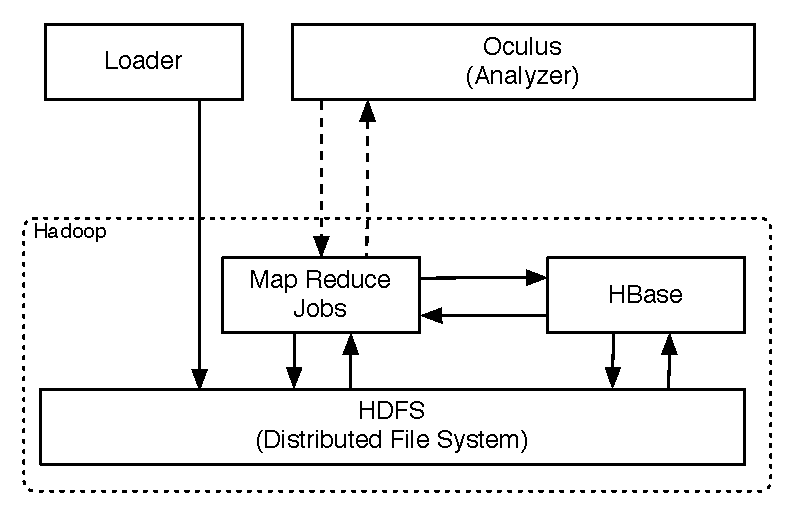
\includegraphics[scale=0.9]{./diagrams/high-level-system.pdf}
  \caption{High level overview of the system's architecture}
  \label{fig:system-overview}
\end{figure}

\section{Loader}
The downloader is responsible for obtaining as much as possible ,,reference data'', by which I mean video material -- from sites such as \textit{youtube.com} or video hosting sites.

It should be also noted that while I refer to this system as ,,the'' downloader, in fact it is composed out of many instances of the same application, sharing the common workload of downloading and converting the input data. The deployment diagram on drawing [12] explains the interactions between the nodes.

\subsection{Work sharing in an actor-based cluster}
The Loader system is implemented following the style of ,,Actor model'' style of concurrency \ref{actor-model}.

 ,,message pasing'' style, which means that the work requests to the cluster come in as \textit{messages}, and then are \textit{routed} to an \textit{actor}, who performs the work, and then responds with another message -- in other words, all comunication between Actor instances is performed via messages and there is no shared state between them. 
This also applies to Actor instances residing in the same JVM - for the user of an ,,Actor System'', the location (on which phisical node the actor is actually executing) of an actor remains fully transparent - this has huge gains in terms of load balancing the message execution on the cluster - the router decides who will be notified on which message, the listing \ref{lst:akka-router-smallest-inbox} shows a typical workflow using the so-called ,,smallest inbox'' routing strategy \ref{akkaDocs}.

% TODO replace with a drawing with actors
\begin{lstlisting}[caption={smallest-inbox routing algorithm},label={lst:akka-router-smallest-inbox}]
                                                           ---> [inbox1, size = 3] => YoutubeDownloadActor(1)
 YoutubeCrawlerActor -- Msg(url=http://...) --> router ---/
                                                          \     [inbox2, size = 5] => YoutubeDownloadActor(2)
                                                                   
                                  /* because inbox1.size < inbox2.size */ 
\end{lstlisting}

The underlying Actor System is implemented by a project called Akka \ref{akkaDocs}, and can be easiest explained as ,,porting Erlang concepts of the Actor Model to the JVM''. I selected the ,,Smallest Inbox'' routing strategy instead of the other widely used ,,Round Robin'' approach in order to guarantee not overloading any Actor with too many requests to download movies (which is a relatively slow process). Thanks to the smallest inbox routing, I can guarantee that if some of the nodes have a faster connection to the Internet, they will get more movie download requests, than nodes located on a slower network.

As mentioned before, the system is fully distributed and \textit{any node can perform any task} submited to the cluster. For example let's take the first step in the processing pipeline in Oculus, which is \verb|Download video from http://www.youtube.com/watch?v=-X9bcrJ3TjY| -- such message will be emited by the \verb|YoutubeCrawlerActor| and sent via a \verb|Router| instance to an \verb|YoutubeDownloadActor| which has the ,,smallest inbox''.


\section{Job Runner}
The job runners responsibility is at the core of the systems... \todo{finish me}

\subsection{Tackling the ,,small-files problem'' on HDFS}
In this section I will explain the ,,small-files problem'' which would lead to major performance degradation of the Hadoop cluster is left undressed, and how I solved it in the reference system -- Oculus.

The so called ,,\textit{small files problem}'' is a known problem in the Hadoop world relating to how HDFS stores files. 
The problem arises whenever we try to store files smaller than the block size used by HDFS to allocate files. One can think of it as wasting space -- because Hadoop allocates at least one block per file we store in it, and all operations (such as migrating data between nodes, reading files into memory etc.) are optimised towards larger block-sizes (usually around 32MB or 64MB). 

To illustrate the problem with an example: if we try storing a 2MB file in HDFS we'll in fact produce 62MB of ,,wasted space'', reducing the cluster's capacity way faster than we ought to. Another p